\documentclass{article}

\usepackage{graphicx}
\usepackage{tikz}
\usepackage{tikzsymbols}
\usetikzlibrary{calc,patterns,shapes.geometric}
\pagestyle{empty}
\usepackage[margin=0pt]{geometry}
\geometry{papersize={14in,12in}}

\def\centerarc[#1](#2)(#3:#4:#5){\draw[#1] ($(#2)+({#5*cos(#3)},{#5*sin(#3)})$) arc (#3:#4:#5);}

\begin{document}
	\begin{figure}
		\centering
		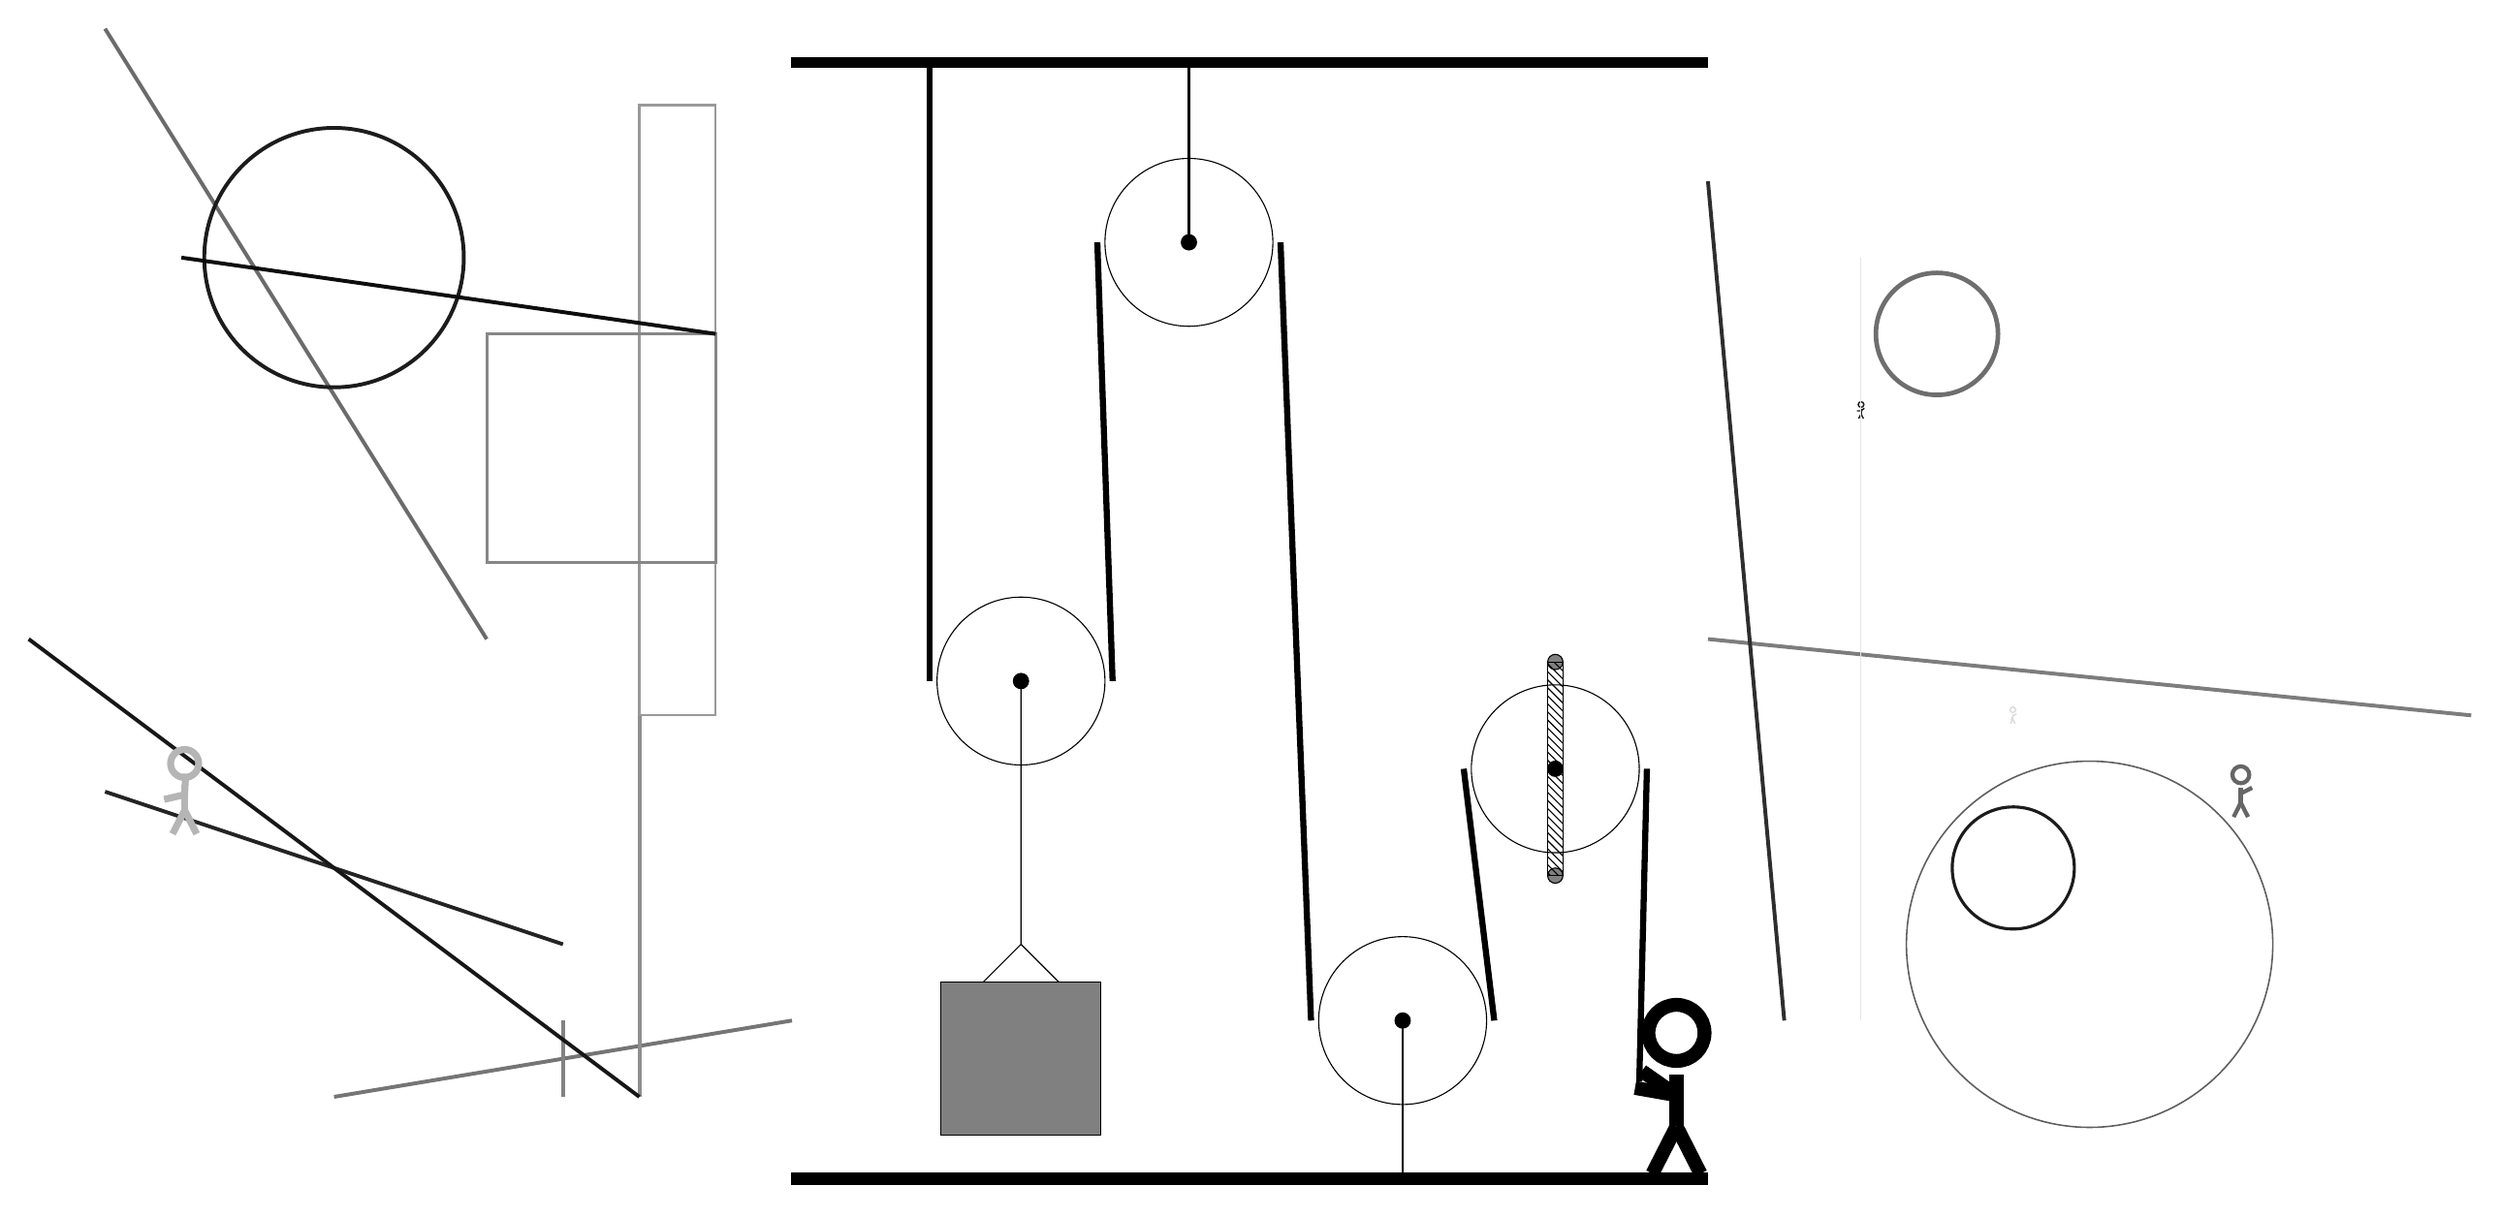
\begin{tikzpicture}
			%%%%% START %%%%%
			
			\draw[fill=black] (-2, 11.5) rectangle (10, 11.625);
			
			\draw[line width=0.5mm, color=black!58](-6, 4) -- (-11, 12);
			
			\draw[line width=0.5mm, color=black!54](-2, -1) -- (-8, -2);
			\draw [line width=0.6mm, color=black!57](13, 8) circle (0.8);
			\draw[line width=0.5mm, color=black!44](-4, 3) -- (-4, -2);
			
			\draw[line width=0.3mm, color=black!40] (-3, 11) rectangle (-4, 3);
			\draw[line width=0.5mm, color=black!49](-5, -1) -- (-5, -2);
			\draw[line width=0.4mm, color=black!47] (-3, 5) rectangle (-6, 8);
			
			\draw[line width=0.5mm, color=black!51](10, 4) -- (20, 3);
			\node[line width=0.4mm, color=black!14] at (14, 3) {\Strichmaxerl[1][69][30]};
			\draw [line width=0.5mm, color=black!89](-8, 9) circle (1.7);
			\draw [line width=0.4mm, color=black!89](14, 1) circle (0.8);
			\draw[line width=0.5mm, color=black!86](-5, 0) -- (-11, 2);
			\node[line width=0.4mm, color=black!60] at (17, 2) {\Strichmaxerl[3][86][27]};
			\draw[line width=0.5mm, color=black!91](-4, -2) -- (-12, 4);
			\node[line width=0.2mm, color=black!89] at (12, 7) {\Strichmaxerl[1][1][38]};
			\draw[line width=0.2mm, color=black!10] (12, -1) rectangle (12, 9);
			
			\draw[line width=0.5mm, color=black!95](-3, 8) -- (-10, 9);
			
			\node[line width=0.7mm, color=black!29] at (-10, 2) {\Strichmaxerl[5][13][87]};
			\draw[line width=0.5mm, color=black!82](10, 10) -- (11, -1);
			
			\draw [line width=0.2mm, color=black!63](15, 0) circle (2.4);
			
			\draw (1, 3.45) circle (1.1);
			\draw[fill=black] (1, 3.45) circle (0.1);
			
			\draw (3.2, 9.2) circle (1.1);
			\draw[fill=black] (3.2, 9.2) circle (0.1);
			\draw[thick] (3.2, 9.2) -- (3.2, 11.5);
			
			\draw (6, -1) circle (1.1);
			\draw[fill=black] (6, -1) circle (0.1);
			\draw[thick] (6, -1) -- (6, -3);
			
			\draw[fill=white](8, 2.3) circle (1.1);
			\draw[fill=black] (8, 2.3) circle (0.1);
			\draw[fill=black!50] (8, 3.7) circle (0.1);
			\draw[fill=black!50] (8, 0.9) circle (0.1);
			\draw[pattern=north west lines, pattern color=black] (7.9, 3.7) rectangle (8.1, 0.9);
			
			\draw (1, 3.45) -- (1, 0.0) -- (0.5, -0.5);
			\draw (1, 0.0) -- (1.5, -0.5);
			\draw[fill=black!50] (-0.05, -0.5) rectangle (2.05, -2.5);
			
			\draw[line width=0.8mm] (-0.2, 11.5) -- (-0.2, 3.45);
			\centerarc[line width=0.8mm](1, 3.45)(180:360:1.2000000000000002);
			\draw[line width=0.8mm](2.2, 3.45) -- (2.0, 9.2);
			\centerarc[line width=0.8mm](3.2, 9.2)(0:180:1.2000000000000002);
			\draw[line width=0.8mm](4.4, 9.2) -- (4.8, -1);
			\centerarc[line width=0.8mm](6, -1)(180:360:1.2000000000000002);
			\draw[line width=0.8mm](7.2, -1) -- (6.8, 2.3);
			\centerarc[line width=0.8mm](8, 2.3)(0:180:1.2000000000000002);
			\draw[line width=0.8mm](9.2, 2.3) -- (9.1, -1.8);
			
			\node at (9.5, -1.9) {\Strichmaxerl[10][-35][170]};
			
			\draw[fill=black] (-2, -3) rectangle (10, -3.15);
			
			%%%%% END %%%%%
		\end{tikzpicture}
	\end{figure}	
\end{document}